
\section{Downloading the Code}

\iamr\ is built on top of the \amrex\ framework.  In order to run
\iamr\, you must download separate git modules for \iamr and \amrex.

\vspace{.1in}

\noindent First, make sure that {\tt git} is installed on your machine.

\vspace{.1in}

\begin{enumerate}

\item Download the \amrex\ repository by typing: 
\begin{verbatim}
git clone https://github.com/AMReX-Codes/amrex.git
\end{verbatim}

This will create a folder called {\tt amrex/} on your machine.
Set the environment variable, {\tt AMREX\_HOME}, on your
machine to point to the path name where you have put \amrex.
You can add this to your {\tt .bashrc} as:
\begin{verbatim}
export AMREX_HOME="/path/to/amrex/"
\end{verbatim}

\item Download the \iamr\ repository by typing: 
\begin{verbatim}
git clone https://github.com/AMReX-Codes/IAMR.git
\end{verbatim}

This will create a folder called {\tt IAMR/} on your machine.

\item You will want to periodically update each of these repositories
by typing {\tt git pull} within each repository.

\end{enumerate}

%\clearpage

\section{Building the Code}

We build the source code in the {\tt IAMR/Exec/run2d/} (for 2D problems) and {\tt IAMR/Exec/run3d/} 
(for 3D) directories.
Example problems with embedded boundaries are in the {\tt IAMR/Exec/eb\_run2d/} and
{\tt IAMR/Exec/eb\_run3d/} directories.
And {\tt IAMR/Exec/run\_2d\_particles} contains an example with passively advected particles.
A local version of the 
\iamr\ executable is built directly in the run folder.  The name of the executable (generated by the make
system) encodes several of the build characteristics, including dimensionality of the problem,
compiler name, and whether {\tt MPI} and/or {\tt OpenMP} were linked with the executable.
Thus, several different build configurations may coexist simultaneously in a problem folder.

The build system is based on GNU make and is relatively self-contained.  We have accumulated 
specialized building setups over the years for a wide variety of hardware configurations, and 
the system is quite easy to modify to add new machine/OS/compiler types and site-specific 
options (optimizations, cross-compiles, user-maintained includes, module-based strategies, etc).
The system currently supports a wide range of Linux, OSX, Windows (via CYGWIN), AIX and BGL 
configurations. With some luck, your machine will be supported ``out of the box'' -- however, if 
you run into problems and need assistance building on your hardware, contact
Ann Almgren (\url{ASAlmgren@lbl.gov}).

In the following, we step through building a representative \iamr\ executable.
\begin{enumerate}
\item We will work in the folder ({\tt IAMR/Exec/run2d}).
From the folder in which you checked out the {\tt IAMR} git repo, type
\begin{verbatim}
cd IAMR/Exec/run2d/
\end{verbatim}

\item Note that in {\tt run2d/}, in the {\tt GNUmakefile} there are the following options

{\tt DIM = 2} (dimensionality of problem)

{\tt COMP = gnu} (or your favorite C++/F90 compiler suite)

{\tt DEBUG = TRUE} (use {\tt FALSE} for an optimized executable with less error checking)

{\tt USE\_MPI = FALSE} (enable MPI)

{\tt USE\_OMP = FALSE} (enable OpenMP)

{\tt USE\_CUDA = FALSE} (enable CUDA)

Do not set both USE\_OMP and USE\_CUDA to TRUE

If you want to try compilers other than those in the GNU suite, and you find that they don't
work, please let us know.

To build a serial (single-processor) code, set {\tt USE\_MPI = FALSE}.
This will compile the code without the MPI library.  If you want to do
a parallel run, set {\tt USE\_MPI = TRUE}.  In this
case, the build system will need to know about your MPI installation.
This can be done by editing the makefiles in the \amrex\ tree
(see {\tt amrex/Tools/GNUMake.md}).

The resulting executable will look something like {\tt amr2d.gnu.DEBUG.MPI.ex},
suggesting that this is a 2-d version of the code, made with 
{\tt COMP=gnu}, {\tt DEBUG=TRUE}, and {\tt USE\_MPI=TRUE}.

\end{enumerate}

\section{Running the Code}

\begin{enumerate}

\item \iamr\ takes an input file as its first command-line argument.  The file may
contain a set of parameter definitions that will overrides defaults set in the code.
To run \iamr\ with an example inputs file, type:
\begin{verbatim}
./amr2d.gnu.DEBUG.ex inputs.2d.bubble
\end{verbatim}
For an MPI build, you can run in parallel using, e.g.:
\begin{verbatim}
mpiexec -n 4 ./amr2d.gnu.DEBUG.MPI.ex inputs.2d.bubble
\end{verbatim}

\item \iamr\ typically generates subfolders in the current folder that
  are named {\tt plt00000/}, {\tt plt00010/}, etc, and {\tt chk00000/},
  {\tt chk00010/}, etc. These are ``plotfiles'' and ``checkpoint''
  files. The plotfiles are used for visualization of derived fields; the checkpoint
  files are used for restarting the code.

  The output folders contain a set of ASCII and binary files.  The field
  data is generally written in a self-describing binary format; the 
  ASCII header files provide additional metadata to give AMR context to the field data.

\end{enumerate}

\section{Visualization of the Results}
\label{sec:visBuild}

There are several options for visualizing the data.  The popular
\visit\ package supports the \amrex\ file format natively, as does
the \yt\ python package and ParaView. \amrvis\ is a package developed
by CCSE that is designed specifically for highly efficient visualization
of block-structured hierarchical AMR data.

\begin{enumerate}

\item Get \amrvis:
\begin{verbatim}
git clone https://ccse.lbl.gov/pub/Downloads/Amrvis.git
\end{verbatim}

Then cd into {\tt Amrvis/}, edit the {\tt GNUmakefile} there
to set {\tt DIM = 2}, and again set {\tt COMP} to the compiler
suite you have. Leave {\tt DEBUG = FALSE}.

Type {\tt make} to build, resulting in an executable that
looks like {\tt amrvis2d...ex}.

If you want to build amrvis with {\tt DIM = 3}, you must first
download and build {\tt volpack}:
\begin{verbatim}
git clone https://ccse.lbl.gov/pub/Downloads/volpack.git
\end{verbatim}

Then cd into {\tt volpack/} and type {\tt make}.

Note: \amrvis\ requires the OSF/Motif libraries and headers. If you don't have these 
you will need to install the development version of motif through your package manager. 
{\tt lesstif} gives some functionality and will allow you to build the amrvis executable, 
but \amrvis\ may exhibit subtle anomalies.

On most Linux distributions, the motif library is provided by the
{\tt openmotif} package, and its header files (like {\tt Xm.h}) are provided
by {\tt openmotif-devel}. If those packages are not installed, then use the
OS-specific package management tool to install them. 

You may then want to create an alias to {\tt amrvis2d}, for example
\begin{verbatim}
alias amrvis2d /tmp/Amrvis/amrvis2d...ex
\end{verbatim}

\item Return to the {\tt IAMR/Exec/run2d} folder.  You should
  have a number of output files, including some in the form {\tt *pltXXXXX},
  where {\tt XXXXX} is a number corresponding to the timestep the file
  was output.  {\tt amrvis2d <filename>} to see a single plotfile
  (see Figure\ref{Fig:Amrvis}), 
   or {\tt amrvis2d -a plt*}, which will animate the sequence of plotfiles.

  Within \amrvis\ you can change which variable you are
  looking at and/or select a region and click ``Dataset'' (under View)
  in order to look at the actual numbers. You can also export the
  pictures in several different formats under "File/Export".

  We have created a number of routines to convert \amrex\ plotfile data
  other formats (such as MATLAB), but in order to properly interpret 
  the hierarchical AMR data, each tends to have its own idiosyncrasies.
  If you would like to display the data in another format, please let us know
  and we will point you to whatever we have that can help.

\end{enumerate}

\begin{figure}[tb]
\centering
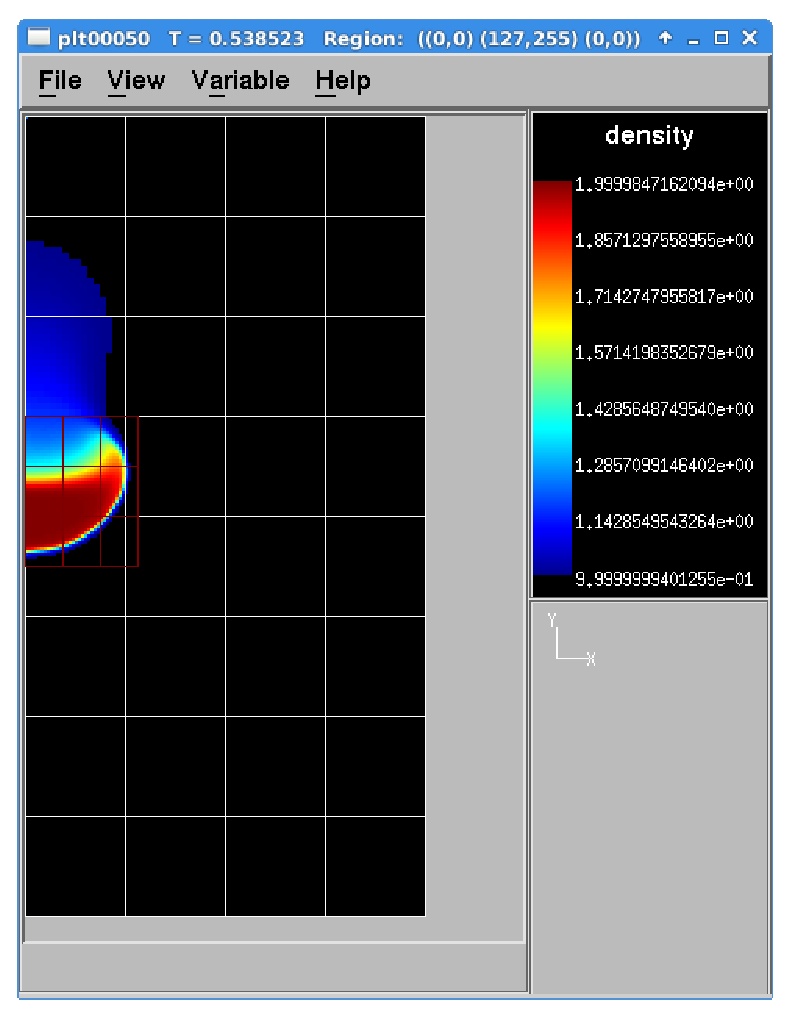
\includegraphics[width=2.5in]{./GettingStarted/IAMR_Plot}
\caption{\amrvis\ visualization tool}
\label{Fig:Amrvis}
\end{figure}

You have now completed a brief introduction to \iamr. 
